\chapter{HAMLET: a Framework for Human-centered AutoML via Structured Argumentation}
\label{human-centric-chap:hamlet}

\begin{figure*}[t]
    \centering
    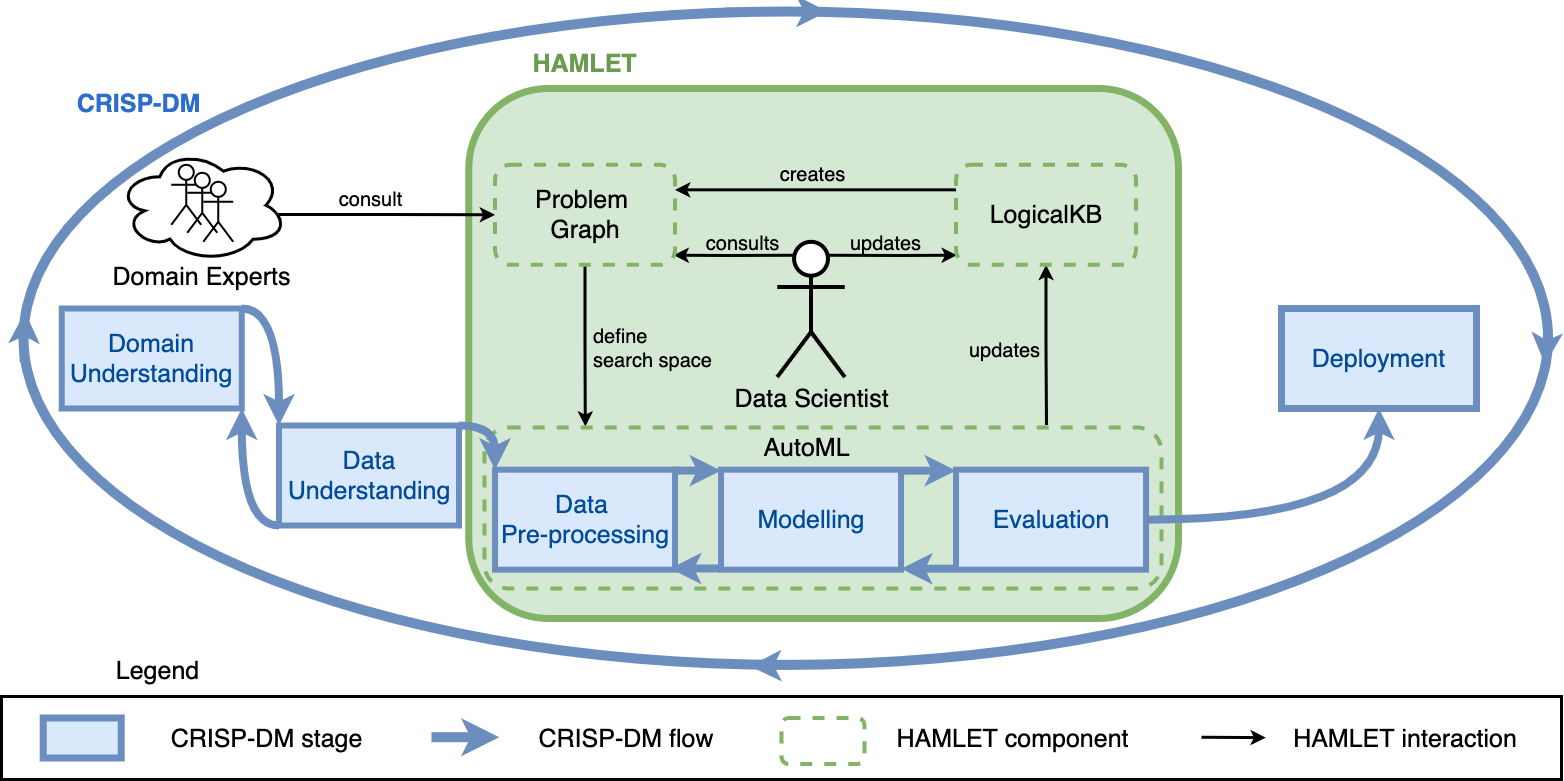
\includegraphics[scale=.25]{chapters/human-centric/hamlet/img/dymmymodel.png}
    \caption{Integrating HAMLET with the CRISP-DM process model.}
    \label{hamlet-fig:approach}
\end{figure*}

% \section{Introduction}\label{intro}
% Data platforms, integrated sets of technologies that collectively meet end-to-end data needs, work towards the automation of data management and analysis \cite{DBLP:journals/fgcs/FranciaGGLRS21}.
% Machine Learning (ML) plays a key role in such processes (e.g., to devise cost models for querying data over heterogeneous data sources \cite{multi-store} and manage data through lineage \cite{dataplat2}; many applications are well surveyed in \cite{zhou2017ml}).
% Data platforms aim at supporting end-to-end data analysis; in this scope, the Cross-Industry Standard Process for Data Mining (CRISP-DM) \cite{wirth2000crisp} is the most acknowledged standard process model---and we will take it as a reference model hencefort.
Given a Machine Learning task to solve, the data scientist collects raw data in arbitrary formats (e.g., from the data lake), builds up knowledge on both the problem and the data, translates such knowledge into \emph{constraints}, designs and trains a model, and finally deploys the solution as a new component integrated into the data platform.
Such a solution consists of a \emph{ML pipeline}.
% : a sequence of \emph{Data Pre-processing transformations} ending with an \emph{ML task}.
The data scientist instantiates the pipeline among a large set of pre-processing transformations and algorithms, which, in turn, can potentially have many \emph{hyperparameters}.
The accuracy of the deployed solution depends on finding both the best algorithms along with their hyperparameters within an exponential search space.

% Automated Machine Learning (AutoML) tools assist the data scientist in finding such an ML pipeline.
% They leverage state-of-the-art optimization approaches to smartly explore huge search spaces of solutions.
AutoML has been demonstrated to provide accurate performance, even in a limited time/iteration budget.
Yet, when setting up the search space, it is highly important for the data scientist to inject her knowledge about the problem into constraints that prevent the AutoML tool from retrieving invalid solutions (i.e., the result of those cannot be deemed correct).
However, the support for constraint/knowledge injection is limited and the AutoML tools became that complex to make it difficult for the data scientist to understand their functioning, hence losing control over the process \cite{XinWLSP21automationml}.

\paragraph{Motivation} The need for a Human-centered and explainable framework for AutoML is real \cite{gil2019towards, lee2020human, wang2019human} (or even mandatory in recent analytic scenarios where the user is interacting with mixed-reality and smart assistants \cite{DBLP:conf/dolap/FranciaGR19,DBLP:journals/is/FranciaGG22}).
It is crucial for the data scientist to augment her knowledge by learning new insights (e.g., new constraints) from the retrieved solutions.
Indeed, the data scientist requires understanding the AutoML process in order to trust the proposed solutions \cite{drozdal2020trust}.
Some works \cite{gil2019towards, lee2020human, wang2019human} prescribe the usage of a Human-centered framework for AutoML, yet they only suggest design requirements.
Alternatively, the authors in \cite{ono2020pipelineprofiler} have proposed a tool that visualizes the best and the worst solutions retrieved by an AutoML tool.
We claim that a Human-centered framework should provide the mechanisms to: (i) help the data scientist to structure her knowledge about the problem in an effective search space; and (ii) augment the knowledge initially possessed by the data scientist with the one produced by the AutoML optimization process.

\paragraph{Contributions} We introduce HAMLET (Human-centered AutoMl via Logic and argumEnTation; \Cref{hamlet-fig:approach}), a framework that enhances AutoML with Structured Argumentation to:
structure the constraints and the AutoML solutions in a Logical Knowledge Base (LogicalKB);
parse the LogicalKB into a human- and machine-readable medium called Problem Graph;
devise the AutoML search space from the Problem Graph;
and leverage the Problem Graph to allow both the data scientist and an AutoML tool to revise the current knowledge.
In this chapter, we commit to the following contributions.
\begin{enumerate}[(i)]
    \item We provide an innovative formalization of the AutoML problem, which considers ML pipelines of multiple lengths, Data Pre-processing steps and user-defined constraints.
    \item We design the formal foundation of HAMLET, supporting the injection of constraints to select ML pipelines as well as the resolution of possible arising inconsistencies.
    \item We implement a functioning prototype of HAMLET.
    \item We provide a preliminary empirical evaluation, including the overhead introduced by the argumentation process and the comparison against state-of-the-art algorithms. 
\end{enumerate}

The remainder of the paper is structured as follows. In \Cref{hamlet-sec:related}, we introduce the related works; we provide the problem formulation in \Cref{hamlet-sec:problem} and its implementation in \Cref{hamlet-sec:implementation}; finally, we provide some preliminary evaluation in \Cref{hamlet-sec:test}, and we draw the conclusions and future research directions in \Cref{hamlet-sec:conclusion}.

\section{Background and Related Works}\label{hamlet-sec:related}
HAMLET intersects two research areas, \emph{human-centric Automated Machine Learning} and \emph{Argumentation}.
In the following, we revise the corresponding related work along with the needed background.
To the best of our knowledge, no contribution lies in this intersection to provide a human-centric approach with argumentation tools.

% \subsection{Automated Machine Learning}
% AutoML tools lighten the data scientist in the overwhelming practice of finding the best ML pipeline instance (AutoML contributions mainly refer to supervised tasks).
% In the early days, only the optimization of the ML task was addressed (but no pre-preprocessing).
% Auto-Weka \cite{kotthoff2019auto} formalized the problem as ``combined algorithm selection and hyperparameter optimization'': various ML algorithms and hyperparameters are tested over a dataset to find the most performing configuration. Such optimization was successfully implemented by leveraging Bayesian optimization \cite{frazier2018tutorial}, a sequential strategy for global optimization: until a limit (budget) of iterations or time is reached, an increasingly accurate model is built on top of the previously explored configurations.

% Recently, AutoML is no longer limited to optimizing just the ML task, but it also includes Data Pre-processing \cite{Giovanelli2021DOLAP, Quemy19DOLAP}.
% In doing so, Auto-sklearn \cite{feurer2019auto} fixes the arrangement of the transformations a priori, without considering that the most performing arrangement changes according to the problem and dataset at hand.
% However, considering several arrangements translates into larger search spaces that are not easy to explore.

% Several improvements have been made to let AutoML tools explore as many configurations as possible.
% Multi-fidelity methods \cite{falkner2018bohb} (i.e., the use of several partial estimations to boost the time-consuming evaluation process) have been exploited. 
% Meta-learning leverages the previous performance of pipeline instances on a wide range of different datasets to provide several recommendations for the dataset at hand, such as promising pipeline instances (possibly acting as an alternative to Bayesian optimization) and search spaces producing good performance.
% Yet, meta-learning per se performs poorly, because it provides coarse-grained recommendations, while it is beneficial in warm-starting Bayesian optimization (i.e., the suggested pipeline instances are visited at the beginning to boost the convergence process).
% With respect to HAMLET, meta-learning per se is not expressive enough to be considered as an alternative, but can be leveraged as a support in building the LogicalKB (i.e., learning constraints that resulted effective on many similar datasets).

% We believe that the data scientist has the duty to revise and supervise the suggested solutions as well as the process producing them.
% Yet, stacking (more and more) complex mechanisms on top of each other unavoidably led to a less understandable optimization that can be hardly controlled by the data scientist (especially if without a strong computer science background).

\subsection{Human-centered AutoML Approaches}
In current state-of-the-art tools, the data scientist role in AutoML is limited to choosing the dataset to analyze, the validation technique (e.g., cross validation, hold out), and the metric to optimize (e.g., accuracy, F1 score).
AutoML researchers aim at making ML accessible to a wider audience;
this has been addressed first by improving automation and now by improving transparency, which also enables human intervention when needed.
Auto-Weka \cite{kotthoff2019auto} and Auto-Sklearn \cite{feurer2019auto} enables non-expert users to build ML models, but the ``black-box'' can be barely open.
Indeed, as advocated in \cite{drozdal2020trust}, data scientists require to understand the process to trust the proposed solutions.
This direction, named ``Human-centered AutoML'', is pursued by both researchers and companies.

As to research contributions, we found plenty of visualization wrappers.
In \cite{drozdal2020trust}, the authors raise the need of incorporating transparency into AutoML: after a session interview, they discover that -- out of all their proposed features -- model performance metrics and visualizations are the most important information to data scientists when establishing their trust in the proposed solutions.
ATMSeer \cite{wang2019atmseer} provides different multi-granularity visualizations to enable users to monitor the AutoML process and analyze the searched models.
PipelineProfiler \cite{ono2020pipelineprofiler} offers interactive visualizations of the AutoML outputs and enables the reproducibility of the results through a Jupiter notebook.
Other contributions enhance current AutoML techniques towards easier human-interactions by: (i) supporting ethic and fair constraints in Bayesian Optimization through a mathematical encoding \cite{perrone2021fair, yaghini2021human}; (ii) simplifying the usage of AutoML with symbolic annotations \cite{peng2020pyglove} and declarative languages \cite{kraska2013mlbase}; (iii) supporting fast feed-backs from AutoML (i.e., runs that are less time-consuming) by leveraging well-known mechanisms of the DBMS (e.g., lineage optimization) \cite{vartak2015supporting, xin2018accelerating}.
Recently, MILE \cite{lee2020human} has proposed to perform AutoML analysis with an end-to-end framework that reflect a DBMS (i.e., a query language + a lineage optimization).

Companies like Google and IBM are the ones most engaged in boosting the involvement of the human in the loop.
Google Vizer \cite{golovin2017google} and Google Facets\footnote{\url{https://pair-code.github.io/facets/}} are the two main visualization tools.
The former reveals details of the different hyperparameters tried in the optimization \cite{golovin2017google}, and the latter focuses on analyzing the output and recognizes biased AI (e.g., ML models that discriminate on sensible attributes such as gender).
As to IBM, AutoAI \cite{wang2020autoai} and AutoDS \cite{wang2021autods} are the tools developed within the MIT-IBM Watson AI Lab.
Specifically, the former enables non-technical users to define and customize their business goals as constraints. 
The latter assists the data scientist team throughout the CRISP-DM process (e.g., in data collection and pipeline design \cite{muller2019data, wang2021autods} and in the augmentation of the DS's knowledge about the dataset features \cite{drozdal2020trust}).

Overall, several studies have been made to understand the proper design of a Human-centered AutoML tool.
In \cite{pfisterer2019towards}, the authors overview the main AutoML issues; while in \cite{khuat2022roles} authors suggest improvements towards the Human-centered shift.
In \cite{gil2019towards, XinWLSP21automationml, crisan2021fits}, interviews with data scientists are conducted to reveal their perception of AutoML as well as their needs and expectations in the next-generation tools.
The main insight is that the future of data science work will be a collaboration between humans and AI systems, in which both automation and human expertise are indispensable \cite{wang2019human}.
To this end, AutoML should focus on: simplicity, reproducibility, and reliability \cite{XinWLSP21automationml, crisan2021fits}.

While the above-mentioned papers mainly focus on visualization, HAMLET brings the data scientist in the loop by allowing her to inject knowledge in the form of constraints, optimizing and learning new constraints through AutoML, and managing such constraints and conflicts through Argumentation.

\subsection{Logic and Argumentation}\label{logic}
Logic is defined as the abstract study of statements, sentences and deductive arguments \cite{Paulson2018logichistory}.
From its birth, it has been developed and improved widely, now including a variety of formalisms and technologies.

Argumentation is a well-known formal tool for handling conflicting information (e.g., opinions and empirical data).
In Abstract Argumentation \cite{Dung1995abstractArg}, a scenario (e.g., a legal case) can be represented by a directed graph.
Each node represents an argument, and each edge denotes an attack by one argument on another. Each argument is regarded as atomic. There is no internal structure to an argument. Also, there is no specification of what is an argument or an attack. A graph can then be analyzed to determine which arguments are acceptable according to some general criteria (i.e., semantics) \cite{baroniCG11semantics}.

A way to link Abstract Argumentation and logical formalisms has been advanced in the field of Structured Argumentation \cite{BesnardGHMPST14structured}, where we assume a formal logical language for representing knowledge (i.e., a LogicalKB) and for specifying how arguments and conflicts (i.e., attacks) can be derived from that knowledge. 
In the structured approach, the premises and claims of the argument are made explicit, and the relationship between them is formally defined through rules internal to the formalism.
We can build the notion of attack as a binary relation over structured arguments that denotes when one argument is in conflict with another (e.g., contradictory claims or premises).
One of the main frameworks for Structured Argumentation is ASPIC\textsuperscript{+}\cite{Modgil2014aspic+}.
In this formalism, arguments are built with two kinds of inference rules: strict rules, whose premises guarantee their conclusion, and defeasible rules, whose premises only create a presumption in favor of their conclusion.
Then conflicts between arguments can arise from both inconsistencies in the LogicalKB and the defeasibility of the reasoning steps in an argument (i.e., a defeasible rule used in reaching a certain conclusion from a set of premises can also be attacked).

Once defined the right logical language for encoding the data scientist and AutoML knowledge, a Structured Argumentation model (e.g., an ASPIC\textsuperscript{+} instance \cite{arg2p-jlc}) can support HAMLET with the formal machinery to build an Argumentation framework upon the data, while Abstract Argumentation would dispense the evaluation tools.

\section{Problem Formulation}\label{hamlet-sec:problem}

\Cref{hamlet-fig:approach} illustrates the overview of HAMLET.
When addressing end-to-end data analysis, a data scientist usually follows a process model such as CRISP-DM.
The data scientist starts by collecting raw data in an arbitrary format.
Then, domain understanding is conducted.
The data scientist works in close cooperation with domain experts and enlists \emph{domain-related constraints} (i.e., intrinsic of the problem).
Follows data understanding, devoted to data analysis, and to extract \emph{data-related constraints} (e.g., defined by the data format).
Domain and data understanding might be repeated many times until the data scientist is satisfied by the acquired knowledge.
Once confident, the data scientist investigates different solutions throughout data pre-processing, modelling, and evaluation.
Data pre-processing and modelling are conducted to effectively build the solution, while evaluation offers a way to measure its performance.
Such a solution consists of a ML pipeline: a sequence of pre-processing steps ending with an ML algorithm that tackles the task.
The data scientist instantiates different pipelines among a large set of transformations and algorithms; the performance are affected by both their implementation and some exposed hyperparameters.
While seeking the best performing and valid solution, the data scientist should consider the already known constraints -- domain- and data-related -- and the ones she discovers during data pre-processing and modelling, respectively: \emph{transformation-} and \emph{algorithm-related constraints} (e.g., due to the intrinsic semantic of transformations and algorithms at hand).
Finally, the process concludes with the deployment of the solution.

HAMLET intersects CRISP-DM, allowing the data scientist to inject and augment her knowledge while automatizing the exploration towards the solution (i.e., instantiate the best ML pipeline). 
We now dig the foundation of HAMLET by incrementally introducing the concepts necessary to move from AutoML to Logic and Argumentation.
% To support the reader, we summarize the main notation in \Cref{hamlet-tbl:symbols}.

\begin{table}[t]
    \centering
    \footnotesize
    \caption{Main symbols used in the formalization.}
    \begin{tabular}{cl}
        \toprule
        \textbf{Symbol} & \textbf{Meaning} \\
        \midrule
        $A$ & Algorithm \\
        $h$ & Algorithm hyperparameter \\
        $S$ & Step \\
        $P$ & Pipeline \\
        $\lambda_*$ & Instance of * \\
        $\Lambda_*$ & Domain of * \\
        $\Lambda$ & Search space \\
        \bottomrule
    \end{tabular}
    \label{hamlet-tbl:symbols}
\end{table}

\subsection{AutoML Formalization}
We provide a novel formalization necessary to move from single algorithms to the optimal pipeline.
For the sake of clarity, we refer to a Classification task, but the formalization also holds for supervised ML tasks in general. % regression tasks.

\begin{definition}[Dataset]
A \emph{dataset} $X$ is a matrix where data items (i.e., rows) are characterized by features (i.e., columns).
\end{definition}

\begin{definition}[Algorithm]
An \emph{algorithm} $A$ is a function that transforms an input dataset $X'$ into a new dataset $X''$.
The algorithm exposes a (possibly empty) set $H$ of \emph{hyperparameters}.
Each hyperparameter $h \in H$ has a \emph{domain} $\Lambda_h$.
We call the \emph{algorithm domain} $\Lambda_A$ the Cartesian product of all hyperparameter domains (i.e., $\Lambda_A = \Lambda_{h_1} \times \ldots \times \Lambda_{h_{|H|}}$).
We call \emph{algorithm instance} $\lambda_A \in \Lambda_A$ an algorithm whose hyperparameters have been assigned with values from their respective domains.
\end{definition}

A Classification algorithm returns a vector (i.e., a matrix with a single column) of labels $Y$ out of the input dataset $X'$.

\begin{definition}[Step]
A \emph{step} $S$ is a set of alternative algorithms with the same goal.
The \emph{step domain} is defined as a disjoint union of the algorithm domains $\Lambda_S = \Lambda_{A_1} \cupdot \ldots \cupdot \Lambda_{A_{|S|}}$.
\end{definition}

Where $\cupdot$ combines the domains of the given algorithms, while retaining the original domain membership (i.e., it is possible to refer to the domain of each algorithm included in a step).

We identify two types of steps: Data Pre-preprocessing steps (e.g., Discretization, Normalization) shape the dataset for the last mandatory step, which fulfill the task---Classification in this case.

\begin{example}[Algorithm and step]
Examples of steps are Normalization ($\altmathcal{N}$), Discretization ($\altmathcal{D}$), and Classification ($\altmathcal{C}l$). 
An algorithm for Classification is Decision Tree  ($\altmathcal{D}t$) \cite{DBLP:books/wa/BreimanFOS84},
examples of hyperparameters for $\altmathcal{D}t$ are its maximum $\textup{depth}$ $(\mathbb{N}^+)$ and the minimum $\textup{samples split}$ $(\mathbb{N}^+)$ required to split a node; hence $\Lambda_{\altmathcal{D}t} = \mathbb{N}^+ \times \mathbb{N}^+$.
An example of algorithm instance is $\lambda_{\altmathcal{D}t}= \{ \textup{depth}=3,\textup{samples\_split}=10 \}$.
\end{example}

\begin{definition}[Pipeline]
Given a (possibly empty) set of Pre-processing steps $\altmathcal{S} = \{S_1,\ldots, S_{|\altmathcal{S}|}\}$ and a Classification algorithm $A$ from the Classification step, a \emph{pipeline} $P$ is a sequence that concatenates steps from $\altmathcal{S}$ and $A$.
The domain of a pipeline is $\Lambda_P = \Lambda_{S_1} \times \ldots \times \Lambda_{S_{|\altmathcal{S}|}} \times \Lambda_A$.
We call \emph{pipeline instance} $\lambda_P$ a sequence of algorithm instances $\lambda_P = \langle \lambda_{A_1}, \ldots, \lambda_{A_{|P|}} \rangle$ such that $\lambda_P \in \Lambda_P$.
\end{definition}

\begin{example}[Pipeline and pipeline instance]
Given the pre-processing steps Normalization ($\altmathcal{N}$) and Discretization ($\altmathcal{D}$), the possible pipelines for the DecisionTree ($\altmathcal{D}t$) are:
\begin{align*}
    P_1 &= \langle \altmathcal{D}t \rangle &
    P_2 &= \langle \altmathcal{D}, \altmathcal{D}t \rangle & 
    P_4 &= \langle \altmathcal{D}, \altmathcal{N}, \altmathcal{D}t \rangle \\
    &&
    P_3 &= \langle \altmathcal{N}, \altmathcal{D}t \rangle & P_5 &= \langle \altmathcal{N}, \altmathcal{D}, \altmathcal{D}t \rangle
\end{align*}
Given \textup{Binarizer} ($\altmathcal{B}$) and  \textup{KBinsDiscretizer} ($\altmathcal{K}b$) as algorithms of Discretization ($\altmathcal{D}$), and \textup{MinMaxScaler} ($\altmathcal{M}m$) and \textup{StandardScaler} ($\altmathcal{S}s$) and  as algorithms of Normalization ($\altmathcal{N}$), we provide examples of instances of $P_2$ and $P_4$:
\begin{align*}
    \lambda_{P_2} &= \langle \lambda_{\altmathcal{B}},~ \lambda_{\altmathcal{D}t} \rangle, &\lambda_{P_4} &= \langle \lambda_{\altmathcal{K}b},~ \lambda_{\altmathcal{M}m},~ \lambda_{\altmathcal{D}t} \rangle \\
    \lambda_{\altmathcal{B}}&=\{ \textup{thr}=5.5 \}, &\lambda_{\altmathcal{K}b}&=\{ \textup{n\_bins}=3, \ldots \}\\
    \lambda_{\altmathcal{M}m}&=\{ \varnothing \}, &\lambda_{\altmathcal{D}t}&= \{ \textup{depth}=3,\ldots\}
\end{align*}
\Cref{hamlet-fig:space} depicts the pipeline domain $\Lambda_{P_4}$ and the pipeline instance $\lambda_{P_4}$.
\label{ex:pipelineinstance}
\end{example}

Depending the on the involved algorithms, their order and hyperparameters, the search space -- out of which the best pipeline instance is select -- is defined as follows.
While, its extraction is later discussed in \Cref{spacealgorithm}.

\begin{definition}[Search space]
The \emph{search space} $\Lambda$ is the Cartesian product of the domain of the Classification step and the disjoint union of the all partial permutations of the pre-preprocessing steps domains.
\end{definition}

AutoML optimizes the exploration of such space.
However, it is not only about algorithms and hyperparameters but also about constraints.

\begin{definition}[Constraint]\label{constraints}
A \emph{constraint} $C \subseteq \Lambda$ is a region of search space that is either \emph{mandatory} or \emph{forbidden}.
Given a pipeline instance $\lambda_P \in \Lambda_P \subseteq \Lambda$
\begin{itemize}
    \item a mandatory constraint $C$ is fulfilled if  $\lambda_P \in C$;
    \item a forbidden constraint $C$ is fulfilled if  $\lambda_P \notin C$.
\end{itemize}
\end{definition}

\begin{figure}
    \centering
    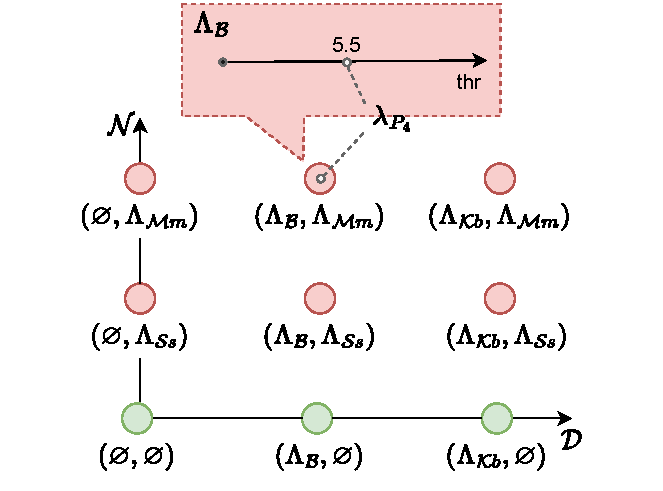
\includegraphics[scale=.75]{chapters/human-centric/hamlet/img/toy_example_ss.pdf}
    \caption{Examples of the pipeline domain $\Lambda_{P_4}$ and pipeline instance $\lambda_{P_4}$, for the sake of visualization we omit the third dimension representing the domain of the Decision Tree. Green (or red) circles represent valid (or invalid) sub-regions of the search space; Normalization is not allowed in the pipeline. The rectangle represents a zoom in the domain of the Binarizer algorithm.}
    \label{hamlet-fig:space}
\end{figure}


\begin{example}[Constraint]
Given the Normalization step ($\altmathcal{N}$) and Decision Tree ($\altmathcal{D}t$) as a Classification algorithm, an example of algorithm-related constraint is ``forbid $\altmathcal{N}$ in pipelines with $\altmathcal{D}t$''.
This discards all the pipelines containing both Normalization and Decision Tree.
\Cref{hamlet-fig:space} depicts the effects of the constraint on the pipeline domain $\Lambda_{P_4}$.
\label{ex:constraints}
\end{example}

Considering all the constraint combinations is overwhelming and, additionally, \emph{conflicts} might occur; for instance in the case of ethical \cite{boston-house} and legal fields that easily inject conflicting constraints into the search space.

\begin{definition}[Constrained pipelines optimization]
Given a search space $\Lambda$ and a set of constraints $\altmathcal{C}$, finding the best pipeline instance $\hat{\lambda}_P$ is defined as $\hat{\lambda}_P = argmax_{\lambda_P \in \Lambda_P} metric(\lambda_P)$, where $metric(\lambda_P)$ is the function evaluating the goodness of $\lambda_P$ and the explored pipelines fulfill the constraints in $\altmathcal{C}$.
\end{definition}

\subsection{Argumentation Formalization}

AutoML is not explainable, hence it does not provide the data scientist with feedbacks that would help her to augment the knowledge about the problem.
It is necessary to represent both (i) the data scientist knowledge about the problem and (ii) the outcome of the AutoML tool in a uniform human-readable medium.
The former helps to drive the optimization process,
the later augments the knowledge about the problem by learning from the explored configurations of pipeline instances---deriving new constraints that increase the data scientist awareness.
We leverage Logic as the key element in defining a common structure (i.e., a uniformed human- and machine-readable medium) on which the knowledge of both the data scientist and the AutoML tool can be combined fruitfully.
In a way, our approach follows the steps of the well known logical based expert systems, of which it is possible to find a great number of successful examples \cite{tan17es}.
Logic provides the tools to cope with one of the distinctive features of the knowledge we want to deal with: inconsistency. Indeed, the ML process is the product of possible attempts, validated or refuted by a consequent evaluation. Hence, the mechanism used to encode the knowledge is required to manage this constant revision process.
This is the role of Argumentation---one of the main approaches for dealing with inconsistent knowledge and defeasible reasoning. 

\begin{definition}[Argumentation Theory]\label{system}
An Argumentation theory is a tuple AS=$\langle L, R \rangle$ with:
\begin{itemize}
    \item $L$ an Argumentation language;
    \item $R$ the set of defeasible rules in the form $r : \phi_0,\ldots, \phi_n \Rightarrow \phi$, where $\phi_0,\ldots, \phi_n,\phi$ are well-formed formulae in the $L$ language and $r$ is the identifier of the rule; we call $\phi_0,\ldots, \phi_n$ the premises of the rule, and $\phi$ its conclusion.
    Rules with no premises are allowed (i.e. $r : \Rightarrow \phi$).
\end{itemize}
\end{definition}

The set of rules $R$ in the theory is used to define how elements from the language are combined together.
In the following two definitions, we specialize $L$ into the language $L_{ML}$ expressing all the basic elements of an AutoML problem and $R$ into a Logical Knowledge Base written in the language $L_{ML}$.

\begin{definition}[AutoML language]
Given an argumentation language $L$, we define the \emph{AutoML language} $L_{ML}$ as $L \cup W$, with $W$ the following set of predicates\footnote{For the sake of conciseness, when writing statements of the AutoML language, the letters $S$ (and $A$) refer to the name of the step (and algorithm)}:
\begin{itemize}
    \item step($S$) with $S \in L$, representing a step $S$ in the pipeline;
    \item algorithm($S$, $A$) with $S, A \in L$, representing an algorithm $A$ for the step $S$;
    \item hyperparameter($A$, $h$, $t$) with $A, h, t \in L$, representing an hyperparameter $h$ for the algorithm $A$ of type $t$ (e.g., numerical, categorical);
    \item domain($A$, $h$, $\Lambda_h$) with $A, h, \Lambda_h \in L$, representing an hyperparameter $h$ for the algorithm $A$ with domain $\Lambda_h$;
    \item pipeline($\langle S_1, \ldots, S_n \rangle$, $A$) with $S_1, \ldots, S_n, A \in L$, representing a pipeline consisting of the sequence of steps $\langle S_1, \ldots, S_n \rangle$ and the Classification algorithm $A$;
    \item mandatory($\langle S_1, \ldots, S_n \rangle$, $Z$) with $S_1, \ldots, S_n, Z \in L$, representing a constraint imposing the steps $\langle S_1, \ldots, S_n \rangle$ on the pipelines with algorithm $A$ ($Z = A$) or on all the Classification pipelines ($Z = \altmathcal{C}l$);
    \item forbidden($\langle S_1, \ldots, S_n \rangle$, $Z$) with $S_1, \ldots, S_n, Z \in L$, representing a constraint forbidding the steps $\langle S_1, \ldots, S_n \rangle$ on the pipelines with algorithm $A$ ($Z = A$) or on all the Classification pipelines ($Z = \altmathcal{C}l$);
    \item mandatory\_order($\langle S_1, \ldots, S_n \rangle$, $Z$) with $S_1, \ldots, S_n, Z \in L$, representing a constraint imposing the sequence of steps $\langle S_1, \ldots, S_n \rangle$ on the pipelines with algorithm $A$ ($Z = A$) or on all the Classification pipelines ($Z = \altmathcal{C}l$).
\end{itemize}
\end{definition}

\begin{definition}[Logical Knowledge Base]
Given the language $L_{ML}$, we call Logical Knowledge Base (LogicalKB) the set of rules for a given AutoML problem.
\end{definition}


In other words, the data scientist leverages an intuitive logical language (i.e., $L_{ML}$), and enlists the constraints one-by-one (i.e., in the LogicalKB).
In our vision, the LogicalKB consists of (i) a set rules specified by the data scientist and a (ii) set of common rules that enable the automatic derivation of pipelines and constraints.
Besides, the data scientist community could create a shared LogicalKB derived from the available literature and similar real-case problems.

\begin{example}[Logical Knowledge Base]\label{ex:kb}
We focus on Discretization ($\altmathcal{D}$),  Normalization ($\altmathcal{N}$) and Classification ($\altmathcal{C}l$) steps, and, for brevity, only define the Classification algorithms: Decision Tree ($\altmathcal{D}t$) and K-Nearest Neighbors ($\altmathcal{K}nn$).
\begin{lstlisting}[mathescape=true]
# define Discretization step
s1 : $\Rightarrow$ step($\altmathcal{D}$).
# define Normalization step
s2 : $\Rightarrow$ step($\altmathcal{N}$).
# define Classification step
s3 : $\Rightarrow$ step($\altmathcal{C}l$).
# DT is a Classification algorithm
a1 : $\Rightarrow$ algorithm($\altmathcal{C}l$, $\altmathcal{D}t$).
# Knn is a Classification algorithm
a2 : $\Rightarrow$ algorithm($\altmathcal{C}l$, $\altmathcal{K}nn$).
# Forbid Normalization when using DT
c1 : $\Rightarrow$ forbidden($\langle\altmathcal{N}\rangle$, $\altmathcal{D}t$).
\end{lstlisting}
\noindent \texttt{s1}, \texttt{s2}, and \texttt{s3} represent the steps; \texttt{a1} and \texttt{a2} represent the algorithms; finally, \texttt{c1} represent the algorithm-related constraint from \Cref{ex:constraints}, namely ``forbid $\altmathcal{N}$ in pipelines with $\altmathcal{D}t$''.
\end{example}

\begin{figure*}
    \centering
    \begin{subfigure}[b]{0.3\textwidth}
        \centering
        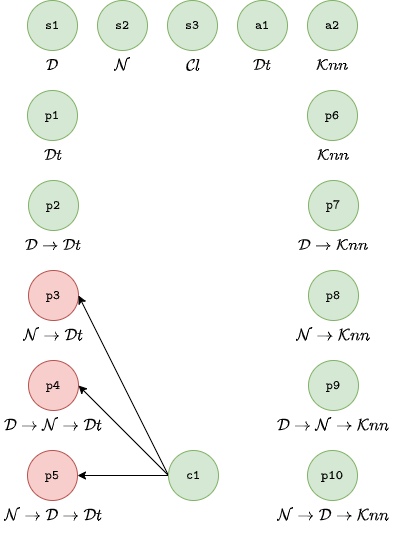
\includegraphics[width=\textwidth]{chapters/human-centric/hamlet/img/toy_example1.png}
        \caption{}
        \label{hamlet-fig:running_a}
    \end{subfigure}
    \hfill
    \begin{subfigure}[b]{0.3\textwidth}
        \centering
        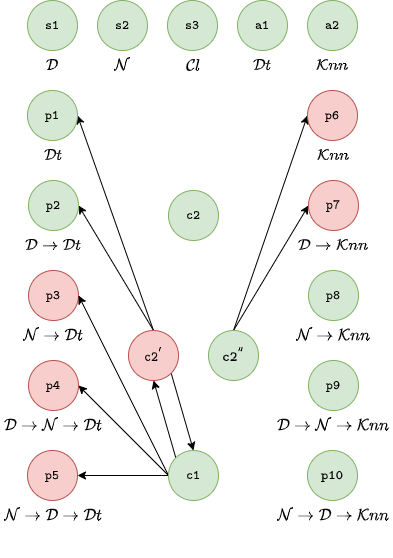
\includegraphics[width=\textwidth]{chapters/human-centric/hamlet/img/toy_example2.png}
        \caption{}
        \label{hamlet-fig:running_b}
    \end{subfigure}
    \hfill
    \begin{subfigure}[b]{0.3\textwidth}
        \centering
        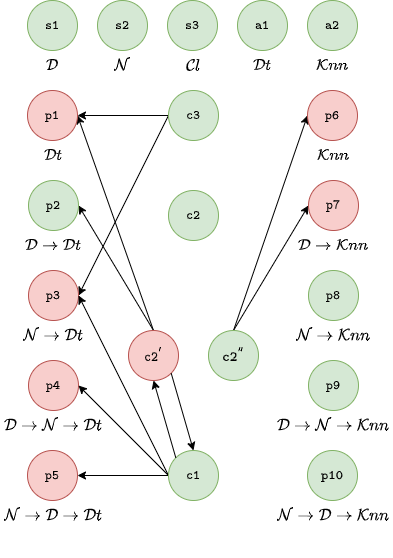
\includegraphics[width=\textwidth]{chapters/human-centric/hamlet/img/toy_example3.png}
        \caption{}
        \label{hamlet-fig:running_c}
    \end{subfigure}
    \caption{Examples of Problem Graphs. Green nodes are valid arguments, red ones are refuted. Arrows are attacks.}
    \label{hamlet-fig:toy_example}
\end{figure*}

When applying constraints, they can be conflicting.
We reify the constraints from \Cref{constraints} through conflict function in the Structured Argumentation domain-

\begin{definition}[AutoML Conflict]\label{conflictauto}
The conflict function $c_{ML}$ is a function from $L_{ML}$ to $2^{L_{ML}}$ that given a statement from $L_{ML}$ returns the set of conflicting statements.
\end{definition}

We support both the AutoML conflicts on ``pipeline vs constraint'' and ``constraint vs constraint''. 
Formally, let us consider two lists of steps $\alpha = \langle \ldots, S_i, S_j, \ldots \rangle$ and $\beta = \langle \ldots, S_y, S_x, \ldots \rangle$.
\begin{itemize}
    \item Pipeline vs constraint: return the constraints conflicting with pipelines.
    \begin{align*}
    c_{ML}&(pipeline(\beta, A)) = \\
        &\{mandatory(\alpha, A)~|~\exists S_i \in \alpha~s.t.~S_i \notin \beta\}~\cup \\
        &\{forbidden(\alpha, A)~|~\forall S_i \in \alpha,~S_i \in \beta \}~\cup\\
        &\{mandatory\_order(\alpha, A)~|~\exists S_i, S_j \in \alpha, S_x, S_y \in \beta, \\&\qquad\qquad\qquad S_i = S_x, S_j = S_y~s.t.~i < j, x > y\}
    \end{align*}
    Intuitively, a pipeline $pipeline(\langle S_i, S_j \rangle, A)$ is conflicting with a $mandatory$ constraint if the pipeline does not contains at least a mandatory step (e.g., the pipeline is conflicting with $mandatory(\langle S_j, S_k \rangle, A)$), with a $forbidden$ constraint if the pipeline contains all the forbidden steps (e.g., the pipeline is conflicting with $forbidden(\langle S_j \rangle, A)$), and with a $mandatory\_order$ constraint if the pipeline contains at least two steps that are not in the mandatory order (e.g., the pipeline is conflicting with $mandatory\_order(\langle S_j, S_i \rangle, A)$).
    \item Constraint vs constraint: return the constraints conflicting with other constraints.
    \begin{align*}
        c_{ML}&(forbidden(\beta, A)) = \{mandatory(\alpha, A)~|~\forall S_j \in \beta, S_j \in \alpha\}\\
        c_{ML}&(mandatory(\beta, A)) = \{forbidden(\alpha, A)~|~\forall S_j \in \alpha, S_j \in \beta\}\\
        c_{ML}&(mandatory\_order(\beta, A)) = \\
        &\{mandatory\_order(\alpha, A)~|~\exists S_i, S_j \in \alpha, S_x, S_y \in \beta, \\&\qquad\qquad\qquad S_i = S_x, S_j = S_y~s.t.~i < j, x > y\}
    \end{align*}
    Intuitively, $mandatory$ and $forbidden$ constraints are in conflict if all the forbidden steps are included in the mandatory constraint (i.e.,  $mandatory(\langle S_i, S_j, S_k \rangle, A))$ and a $forbidden(\langle S_i, S_j \rangle, A))$), this hold symmetrically for $forbidden$ and $mandatory$ constraints. Two $mandatory\_order$ constraints are in conflict if they contain at least two steps in different order (i.e.,  $mandatory\_order(\langle S_i, S_j, S_k \rangle, A))$ and a $mandatory\_order(\langle S_j, S_i \rangle, A))$).
\end{itemize}


\begin{example}[AutoML conflict]
With reference to the LogicalKB in \Cref{ex:kb}, let us consider the set of rules that represent the pipelines related to $\altmathcal{D}t$:
\begin{lstlisting}[mathescape=true]
# pipeline ending with a DT
p1 : $\Rightarrow$ pipeline($\altmathcal{D}t$).
# Discretization and DT
p2 : $\Rightarrow$ pipeline($\langle\altmathcal{D}\rangle$, $\altmathcal{D}t$).
# Normalization and DT
p3 : $\Rightarrow$ pipeline($\langle\altmathcal{N}\rangle$, $\altmathcal{D}t$).
# Discretization, Normalization, and DT
p4 : $\Rightarrow$ pipeline($\langle\altmathcal{D}$, $\altmathcal{N}\rangle$, $\altmathcal{D}t$).
# Normalization, Discretization, and DT
p5 : $\Rightarrow$ pipeline($\langle\altmathcal{N}$, $\altmathcal{D}\rangle$, $\altmathcal{D}t$).
\end{lstlisting}
In this case, \texttt{c1} (i.e., ``forbid $\altmathcal{N}$ in pipelines with $\altmathcal{D}t$'') is in conflict with the \emph{pipeline} statements \texttt{p3}, \texttt{p4}, and \texttt{p5} since they contain $\altmathcal{N}$ and $\altmathcal{D}t$.
\label{ex:conflict}
\end{example}

To create a Problem Graph, which is the medium readable by users and machines, we informally (for the sake of conciseness) introduce the key elements from Structured Argumentation; a complete formalization is available in \cite{Modgil2014aspic+}.
Given an Argumentation theory, an \emph{argument} is created for every rule with no premises (e.g., from the rule $r : \Rightarrow c$, we derive an argument with \emph{conclusion} $c$ using $r$).
Then, we recursively apply the other rules in the theory to the newly generated argument (e.g., we can use the argument with conclusion $c$ and the following rule $r1 : c \Rightarrow d$ to conclude an argument for $d$ using $r$ and $r1$).
This is repeated until no new argument can be generated.
In the rest of the paper we will refer to an argument with the set of rules used to generate it (e.g., given $r : \Rightarrow c$ and $r1 : c \Rightarrow d$, we will write $r$ and $r1$ when referring to the rules and $\{r\}$ and $\{r, r1\}$ for -- respectively -- the argument with \emph{conclusion} $c$ using $r$ and the argument with \emph{conclusion} $d$ using $r$ and $r1$).

An \emph{Argumentation framework} is defined using the arguments built from an Argumentation theory and their \emph{attack} relations.
Attacks are inconsistencies between arguments' conclusions and are computed using a conflict function (\Cref{conflictauto}).
For instance, given two arguments concluding respectively $a$ and $b$, and the conflict function $c$ such that $c(a) = \{b\}$, then the argument for $b$ directly attacks the one for $a$ (i.e., $b$ is in conflict with $a$).
The attack is propagated to all the arguments built over the receiver of the attack (e.g., if $a_1$ directly attacks $a_2$, and $a_2$'s conclusion is used to derive $a_3$, then $a_1$ also attacks $a_3$).
Also, we can define a \emph{preference} relation over arguments using a partial ordering over the rules in the Argumentation theory:
it is impossible for an argument to be attacked by the least preferred ones, even if they are in conflict.
In other words, we can explicitly solve inconsistencies in the LogicalKB using priorities.
We exploit the \emph{last-weakest} ordering as in \cite{Modgil2014aspic+}.

Finally, the evaluation of an Argumentation framework is performed through semantics, which determines all the sets of arguments that are consistent (called \emph{extensions}) in an Argumentation framework.
We exploit grounded semantics \cite{Dung1995abstractArg} to produce a \emph{grounded extension}; this semantics is the most skeptical---i.e., it includes only the arguments that are verified by all the possible interpretations. % of the graph.

\begin{definition}[Problem Graph]
We call \emph{Problem Graph} a graph in which nodes are arguments and edges are attacks from the Argumentation framework that is built on the Argumentation theory $\langle L_{ML}, LogicalKB \rangle$ and the conflict function $c_{ML}$.
\end{definition}

The benefits of the Problem Graph are two-fold.
First of all, it can be leveraged by both data scientists and domain experts to: understand, summarize and visualize the current knowledge.
Second of all, it is straightforward to convert such a graph of constraints into a space of possible solutions (i.e., exploiting Argumentation semantics, it is easy to obtain all the sets of arguments -- constraints and pipelines -- which hold together).

\begin{example}[Problem Graph]
\Cref{hamlet-fig:toy_example}a illustrates the Problem Graph extracted from the LogicalKB introduced in \Cref{ex:kb,ex:conflict} and evaluated under grounded semantics.
Arguments are represented as nodes, attacks as arrows and the colors represent the state of the arguments according to the semantics: red for refuted arguments, and green for the ones in the extension.
The arguments are identified through the set of rules used to build them.
In the upper part of the figure, we have a group of undefeated arguments, namely \texttt{\{s1\}}, \texttt{\{s2\}}, \texttt{\{s3\}}, \texttt{\{a1\}}, and \texttt{\{a2\}}, representing the basic knowledge used to setup the AutoML search space (i.e. steps and algorithms).
Then, we have an argument for every pipeline in \Cref{ex:conflict}: from \texttt{\{p1\}} to \texttt{\{p5\}} the pipelines regarding $\altmathcal{D}t$, from \texttt{\{p6\}} to \texttt{\{p10\}} the ones regarding $\altmathcal{K}nn$.
Finally, we can observe three different attacks: from \texttt{\{c1\}} to \texttt{\{p3\}}, \texttt{\{p4\}}, and \texttt{\{p5\}}, in accordance with the conflicts identified in \Cref{ex:conflict}.
The arguments in the extension give us all the information that we should use during the AutoML optimization process -- i.e. we should discard all the pipelines refuted by the constraint argument ($\{c1\}$), and focus on the remaining part of the search space.
\label{ex:graph}
\end{example}

The use of Argumentation relieves the data scientist of the burden of manually considering all the effects of the possible constraints.
It is important to notice that, although the increased degree of automation, the Problem Graph allows the data scientist and domain experts to correct, revise, and supervise the process.
Accordingly, possible inconsistencies -- due to diverging constraints -- can be verified by the data scientist using her knowledge.

Any change in the LogicalKB translates into a change in the Problem Graph, allowing the data scientist and domain experts to visualize it and argue about it.
The revision of the Problem Graph is the key element in the process of augmenting the knowledge: the data scientist and domain experts can consult each other and discuss how the new insights relate to their initial knowledge.
Indeed, thanks to the nature of the Problem Graph, it would be extremely easy to identify new possible conflicts and supporting arguments.
Furthermore, AutoML can update the Problem Graph by extracting constraints from the performed exploration, and transposing them into the LogicalKB.
For instance, the data scientist may not have considered that the dataset contains missing values.
AutoML helps in identifying the new data-related constraint ``require Imputation ($\altmathcal{I}$) in all the pipelines'' and adds it to the LogicalKB ($mandatory(\langle \altmathcal{I} \rangle, \altmathcal{C}l)$).

The described process is compliant with and augments the CRISP-DM process.
The inferred/learned knowledge is automatically handled throughout iterations, supporting the data scientist in the whole analysis in a continuous revision of the constraints.
\vspace{2cm}

\section{HAMLET}\label{hamlet-sec:implementation}

\begin{figure*}[t]
\begin{lstlisting}[mathescape=true]
# given an algorithm, create a pipeline including only such algorithm
hc0 : algorithm($\altmathcal{C}l$, A) $\Rightarrow$ pipeline($\langle~\rangle$, A).
# given some steps and an algorithm, create a pipeline including such steps and algorithm
hc1 : step($S_1$),$\ldots$,step($S_n$), algorithm($\altmathcal{C}l$, A) $\Rightarrow$ pipeline($\langle S_1, \ldots, S_n \rangle$, A).
# given constraints on the Pre-processing steps required for Classification...
# ... apply this constraints to all Classification algorithms
hc2 : mandatory($\langle S_1, \ldots, S_n \rangle$, $\altmathcal{C}l$), algorithm($\altmathcal{C}l$, A) $\Rightarrow$ mandatory($\langle S_1, \ldots, S_n \rangle$, A).
hc3 : forbidden($\langle S_1, \ldots, S_n \rangle$, $\altmathcal{C}l$), algorithm($\altmathcal{C}l$, A) $\Rightarrow$ forbidden($\langle S_1, \ldots, S_n \rangle$, A).
hc4 : mandatory_order($\langle S_1, \ldots, S_n \rangle$, $\altmathcal{C}l$), algorithm($\altmathcal{C}l$, A) $\Rightarrow$ mandatory_order($\langle S_1, \ldots, S_n \rangle$, A).
\end{lstlisting}
\caption{A subset of rules from the LogicalKB.}
\label{rules-arg2p}
\end{figure*}

HAMLET iterates over three phases (\Cref{hamlet-fig:approach}): (i) the generation of Problem Graph and search space out of the LogicalKB, (ii) the exploration of the search space in compliance with the specified constraints, and (iii) the augmentation of the LogicalKB through a rule recommendation.

The framework is available at \url{https://github.com/QueueInc/HAMLET}, and it is composed of two sub-modules. 
The first, written in Kotlin and running on the JVM, exposes a graphical interface on which the data scientists can compile and revise the LogicalKB. 
The module is also responsible for the generation and evaluation of the Problem Graph; it implements the Structured Argumentation functionalities as specified in \Cref{hamlet-sec:problem} using \argtup{} \cite{arg2p-jlc}, an ASPIC\textsuperscript{+}-based Kotlin library.
The second module, written in Python, is responsible for performing the AutoML optimization and the extraction of the new constraints from the explored space.

\subsection{Generation of Problem Graph and Search Space}
In \Cref{hamlet-sec:problem}, we defined the LogicalKB as the set of rules specified by the data scientist using her knowledge.
The LogicalKB also includes a set of hard-encoded rules representing inferences necessary to characterize the AutoML problems.
These rules are joined to the ones defined by the data scientist and used to build the Problem Graph (i.e., Argumentation framework).

A subset of rules is shown in \Cref{rules-arg2p}.
The first two ($hc0$ and $hc1$) define how to automatically derive a pipeline using algorithms and steps.
The construction of pipelines can be completely automated and the data scientist should be dispensed from manually enumerating all the possible pipelines as in \Cref{ex:conflict}.
In particular, the correct set of rules is built dynamically using the steps and algorithms provided by the DS, then they are used to derive all the arguments for the possible pipelines.
The last three rules ($hc2, hc3$ and $hc4$) encode constraints -- mandatory, forbidden, mandatory\_order -- on all the available algorithms with a single statement (e.g., $mandatory(\langle \altmathcal{D} \rangle, \altmathcal{C}l)$): it will be automatically used by the framework to derive the constraints for all the specific algorithms in the theory.

\begin{example}[Hard-coded rules]
With reference to \Cref{ex:graph} and \Cref{rules-arg2p}, we add rule \texttt{c2} for a new data-related constraint.
\begin{lstlisting}[mathescape=true]
# mandatory Norm. in Class. pipelines
c2 : $\Rightarrow$ mandatory($\langle\altmathcal{N}\rangle$, $\altmathcal{C}l$)
\end{lstlisting}
From the rule \texttt{c2}, the hard-coded rules generate the two arguments
\texttt{c2' = \{c2, a1, hc2\}} (i.e., $mandatory(\langle\altmathcal{N}\rangle, \altmathcal{D}t)$) and \texttt{c2'' = \{c2, a2, hc2\}} (i.e., $mandatory(\langle\altmathcal{N}\rangle, \altmathcal{K}nn)$) that are specific for the Classification algorithms in the LogicalKB.

However, \texttt{\{c1\}} (i.e., $forbidden(\langle\altmathcal{N}\rangle, \altmathcal{D}t)$; is in conflict with \texttt{c2'}.
Depending on her experience, the data scientist decides to resolve the conflict by specifying an ordering over the rules in the LogicalKB.
Assuming that the data scientist prefers \texttt{c1} to \texttt{hc2},
the argument \texttt{\{c1\}} is preferred to \texttt{c2'} and the attack from the latter is not considered in the final graph.
\Cref{hamlet-fig:toy_example}b shows the updated graph.
Firstly, we observe the support relation between \texttt{\{c2\}} and the generated constraints \texttt{c2'} and \texttt{c2''}.
Since \texttt{\{c1\}} has no attackers, it is added to extension.
Consequently, \texttt{c2'} is refuted and the pipelines attacked by it are correctly reinstated.
\label{ex:hard_coded_rules}
\end{example}

Given the Problem Graph (we recall that the Problem Graph contains \emph{all} the generated pipelines -- including their partial permutations), the search space can be extracted as in \Cref{spacealgorithm}. 
We iterate over all the generated pipelines in the Problem Graph and we recursively build their domain: the pipeline domain is the Cartesian product of the step domains, the step domain is the disjoint union of the algorithm domains (we leverage the disjoint union since each algorithm can be picked as an alternative to the others), the algorithm domain is the Cartesian product of its hyperparameters; the domain of a hyperparameter is given by definition.
Finally, the search space is the disjoint union of all the alternative pipeline domains.

Noticeably, while the search space could be constrained during its construction (e.g., by simply adding an ``if'' condition to check the validity of each pipeline at \Cref{spacealgorithm} line 10), current AutoML frameworks leverage optimization techniques that do not allow the explicit exclusion of regions from the search space.
As a consequence, we need to produce the entire search space first.

\begin{algorithm}[t]
\caption{Search Space from the Problem Graph}
\label{spacealgorithm}
\footnotesize
\begin{algorithmic}[1]
\Require{PG(N, E): Nodes and Edges of a Problem Graph}
\Ensure{$\Lambda$: Search Space}
    \item[]
    \Procedure{GetDomain}{$A$}
        \State $\Lambda_A \leftarrow \varnothing$
        \ForEach{$h \in A$} \Comment{For each hyperparameter in the algorithm...}
            \State $\Lambda_A \leftarrow \Lambda_A \times \Lambda_h$ 
            \Comment{Compute Cartesian product of hyperpar. domains}
        \EndFor
        \State \Return $\Lambda_A$ \Comment{Return the algorithm domain}
    \EndProcedure
    \item[]
    \State $\Lambda \leftarrow \varnothing$ \Comment{Initialize the search space}
    \ForEach{$pipeline(\alpha, A) \in N$} \Comment{For each argument that is a pipeline with $\alpha$ steps and alg. $A$...}
        \State $ \Lambda_{P} \leftarrow \textup{GetDomain(A)}$ \Comment{Init. pipeline domain with algorithm domain}
        \ForEach{$S \in \alpha$}  \Comment{For each step in the pipeline...}
            \State $\Lambda_{S}  \leftarrow \varnothing$ \Comment{Init. the step domain}
            \ForEach{$A \in S$}  \Comment{For each algorithm in the step...}
                \State $\Lambda_{S} \leftarrow \Lambda_{S} \cupdot \textup{GetDomain(A)}$ \Comment{Add alg. to step domain}
            \EndFor
            \State $\Lambda_P \leftarrow \Lambda_P \times \Lambda_S$ \Comment{Add step domain to pipeline domain}
        \EndFor
        \State $\Lambda \leftarrow \Lambda \cupdot \Lambda_P$ \Comment{Add pipeline domain to the search space}
    \EndFor
    \State \Return $\Lambda$ \Comment{Return the search space}
\end{algorithmic}
\end{algorithm}

\subsection{Exploration of a Constrained Search Space}\label{subsec:constrained_automl}

The Problem Graph is not only used to build the entire search space but it is also evaluated to understand which pipelines are invalid and which constraints are valid.
Hence -- through the Problem Graph -- we enhance AutoML exploration by combining the following techniques.
\begin{itemize}
    \item[(i)] Invalid pipelines are used to discourage the exploration of such a portion of the search space (we recall that a pipeline has a domain -- a region of the search space -- in which several pipeline instances are parametrized).
    First, we sample such regions of the search space, then we enforce a knowledge injection mechanism through warm-starting (i.e., the process of providing previous evaluations that help the model to converge faster).
    For instance, with reference to \Cref{ex:hard_coded_rules}, we sample some pipeline instances from the pipelines that have been discarded (from \texttt{\{p3\}} to \texttt{\{p7\}});
    then, we label such samples as invalid and provide them to the AutoML tool, helping the optimization algorithm to focus only on the valid portions of the space.
    \item[(ii)] Valid constraints -- expressed as conjunctions of Boolean clauses -- are used to discard the invalid pipeline instances that still are encountered by the AutoML tool.
    Indeed, since the sampling from (i) is non-exhaustive, it can happen that small portions of invalid regions could still be explored.
\end{itemize}

Our AutoML implementation is based on FLAML \cite{wang2021flaml}, which mixes Bayesian Optimization with CFO (Frugal Optimization for Cost-related Hyperparameters).
In a standard Bayesian process, an increasingly accurate model is built on top of the previously explored pipeline instances to suggest the most promising ones among the remaining.
The pipeline instances keep being explored, updating the model, until a budget in terms of either iterations or time is reached.
With CFO, there is also an estimation of the evaluation time to consider the frugality of the suggested pipeline instances -- hence favoring the ones requiring a smaller amount of time.
Throughout the exploration, different solutions are tested, which contribute to augmenting the global knowledge about the problem.

\subsection{Knowledge Augmentation through Rule Recommendation}

New constraints are automatically mined out of the pipeline instances explored by AutoML and \emph{recommended} in our logical language as rules.
Then, the data scientist decides which rules are accepted and added to the LogicalKB.


At this stage, we leverage frequent pattern mining techniques to learn constraints in an unsupervised manner.
Frequent pattern mining is the task of finding the most frequent and relevant patterns in large datasets (e.g., finding the products frequently bought together in the domain of market basket analysis); depending on the constraint type, we look for (sub)sets \cite{srikant1995mining} or (sub)sequences \cite{srikant1996mining} frequently recurring among the explored pipelines.
Since a pipeline instance is a sequence of algorithms, the set of the explored pipeline instances can be directly mapped into a transactional dataset \cite{srikant1995mining} where each pipeline instance is a transaction and each step -- inferred from the algorithm -- is an item.

We recommend the same constraints we support at the Argumentation level (i.e., $mandatory$, $forbidden$, $mandatory\_order$) so that AutoML can be as expressive as the DS.
For mandatory and forbidden constraints we look for (sub)sets \cite{srikant1995mining} frequently recurring among the explored pipelines.
Specifically, we split the explored pipeline instances by the applied Classification algorithm, set a minimum frequency (i.e., support) threshold to 50\% (i.e., to be retrieved, a set/sequence must occur at least in 50\% of the explored instances), and extract frequent maximal\footnote{Maximal itemsets are patterns that are not contained in any other.
For instance, given two frequent patterns, $\{a, b, c\}$ and $\{a, b\}$, the former is maximal while the latter is not.
}
itemsets.
The recommendation depends on the constraint.
\begin{itemize}
    \item $mandatory$: we consider only the patterns with good performance (i.e., $0.7 \leq metric \leq 1.0$); 
    \item $forbidden$: we consider only the patterns with bad performance (i.e., $0.0 \leq metric \leq 0.3$);
    \item $mandatory\_order$: the same considerations of the mandatory constraints stand, except that we look for (sub)sequences \cite{srikant1996mining} of length 2 to discover ordering dependencies in pairs of steps as in \cite{giovanelli2021data}.   
\end{itemize}
We leveraged well-known implementations \cite{raschkas_2018_mlxtend} and \cite{seq2pat2022} for itemsets and sequences mining, respectively.
Finally, we return to the data scientist only the top-10 rules sorted by descending support; we allow the data scientist to explore all the rules on-demand.

The thresholds act as filters on the extracted rules since we cannot burden the user with the investigation of hundreds of recommendations. 
As to the intervals, our rationale is simple: we only want to recommend as mandatory (order) the rules that achieved ``good performance'' and as forbidden the rules that achieved ``bad performance''.
Since we handle classification pipelines that mainly refer to (balanced) accuracy/F1 score/recall, we mapped ``good'' in the interval $[0.7, 1.0]$ and ``bad'' in the interval $[0, 0.3]$. For the frequent pattern extraction, we consider only the pipeline instances falling in these intervals.
As to the support, 50\% ensures that the pattern recurs on many of the explored instances and empirically showed to be a good threshold to have good efficiency in the extraction of frequent patterns.

\begin{example}[Rules Recommendation]
With reference to the Problem Graph in \Cref{ex:hard_coded_rules},
the AutoML results are filtered according to the chosen metric, the algorithm \cite{raschkas_2018_mlxtend} is applied, and let us assume that the rule \texttt{c3} is recommended:
\begin{lstlisting}[mathescape=true]
c3 : $\Rightarrow$ mandatory($\langle\altmathcal{D}\rangle$, $\altmathcal{D}t$).
\end{lstlisting}
The constraints specifies ``mandatory $\altmathcal{D}$ in pipelines with $\altmathcal{D}t$''.
As a matter of fact, it is well known that Discretization improves the performance of tree-based algorithms giving to them the ability to apply multiple split in the decision nodes.
\Cref{hamlet-fig:toy_example}c shows the effect of the applied constraint: a new portion of the search space is excluded from the extension ($\{p1\}$).
\end{example}


\section{Experimental Evaluation}\label{hamlet-sec:test}

The performance of HAMLET depends on (i) the rules encoded in the LogicalKB and (ii) the rules recommended after each run.
To test both the effectiveness and efficiency of our approach, we define three experimental settings.
\begin{itemize}
    \item PKB (Preliminary Knowledge Base), HAMLET starts with a preliminary LogicalKB constraining the search space from the first iteration, and no rule mining is applied.
    %, but the rules that are suggested throughout the iterations are not applied.
    The preliminary LogicalKB consists of the rules discovered in \cite{giovanelli2021data} and some well-known from the literature (e.g., suggested by scikit-learn\footnote{\url{https://scikit-learn.org/stable/auto_examples/preprocessing/plot_discretization.html}}).
    The complete knowledge base can be found in the Github repository.
    \item IKA (Iterative Knowledge Augmentation), HAMLET starts with an empty LogicalKB, and all the rules recommended after each run are applied to extend the LogicalKB.
    \item PKB+IKA, HAMLET starts with a preliminary LogicalKB, and the rules recommended after each run are applied to extend the LogicalKB.
\end{itemize}
HAMLET run 4 times in every setting -- intuitively, four runs of knowledge augmentation -- the budget assigned to each run is 125 pipeline instances in 900 seconds (15 minutes).
We also test against a baseline: we let AutoML explore 500 pipeline instances ($= 125 \cdot 4$) in a single run with a time budget of 3600 seconds ($= 900 \cdot 4$; 1 hour).

For such an evaluation, we derive a search space out of 6 steps, 5 Data Pre-processing steps (Imputation, Normalization, Discretization, Feature Engineering, and Rebalancing) followed by the final Classification task.
Since the tests are run on datasets from OpenML \cite{OpenML2013} -- a well-known repository for data acquisition and benchmarking -- and it provides already-encoded datasets, we do not consider the encoding step. 
Except for that, we included all the Data Pre-processing steps and algorithms available in the scikit-learn \cite{scikit-learn} Python library (plus imbalance-learn \cite{JMLR:v18:16-365} for Rebalancing transformations).
The leveraged steps, algorithms per step, and hyperparameters per algorithm are reported in \Cref{hamlet-tbl:search_space}.

\begin{table}[t]
    \footnotesize
    \caption{Algorithms and number of hyperparameters for each of the steps in HAMLET. Algorithm names and hyperparameters are imported from the scikit-learn Python library.}
    \centering
    \begin{tabular}{llc}
        \toprule
        \textbf{Step} & \textbf{Algorithm} & \textbf{\#Hyperparameters}  \\\midrule
        Imputation        & SimpleImputer & 1 \\
                          & IterativeImputer & 2 \\
        Normalization     & StandardScaler & 2 \\
                          & MinMaxScaler & 0 \\
                          & RobustScaler & 2 \\
                          & PowerTransformer & 0 \\
        Discretization    & Binarizer & 1 \\
                          & KBinsDiscretizer & 3 \\
        Feature Eng.      & SelectKBest & 1 \\
                          & PCA & 1 \\
        Rebalancing       & NearMiss & 1 \\
                          & SMOTE & 1 \\
        Classification    & DecisionTreeClassifier & 7 \\
                          & KNeighborsClassifier & 3 \\
                          & RandomForestClassifier & 7 \\
                          & AdaBoostClassifier & 2 \\
                          & MLPClassifier & 6 \\ \bottomrule
    \end{tabular}
    \label{hamlet-tbl:search_space}
\end{table}

The OpenML-CC18 suite is a well-known collection of 72 datasets for benchmarking.
Given the time-consuming computation of each dataset (8 hours per dataset = 2 hours for the baseline + 6 hours for HAMLET in the three settings) -- in this preliminary evaluation -- we select a representative subset of datasets according to three meta-features provided by OpenML: number of instances, number of features, and number of classes.
For each of the considered meta-features, we search for datasets with either high or low values, and we select the representatives that maximize the overall dataset diversification.
\Cref{hamlet-tbl:datasets} illustrates the 6 datasets that have been identified; note that some combinations of meta-features have no representative dataset in the suite.
Among these, we do not report the results for the dataset mnist\_784 since the number of explored pipeline instances is insufficient to validate the result (i.e., due to the time necessary to run a single pipeline instance, only 50 instances were explored out of 1000).

\begin{table}[t]
    \caption{Dataset descriptions.}
    \footnotesize
    \label{hamlet-tbl:meta_features}
    \begin{threeparttable}
    \centering
        \begin{tabular}{ll|ll|ll|ll}
            \toprule
             \textbf{OpenMLID} \tnote{a} & \textbf{Dataset} & \multicolumn{2}{c}{\textbf{Instances}} & \multicolumn{2}{c}{\textbf{Features}} & \multicolumn{2}{c}{\textbf{Classes}}  \\ \midrule
             40983 & wilt & 4839 & \footnotesize{\texttt{L}} & 6 & \footnotesize{\texttt{L}} & 2 & \footnotesize{\texttt{L}}\\
             40499 & texture & 5500& \footnotesize{\texttt{L}} & 41& \footnotesize{\texttt{L}} & 11& \footnotesize{\texttt{H}}\\
             1485 & madelon & 2600 & \footnotesize{\texttt{L}} & 501 & \footnotesize{\texttt{H}} & 2 & \footnotesize{\texttt{L}}\\
             1478 & har & 10229 & \footnotesize{\texttt{L}} & 562& \footnotesize{\texttt{H}} & 6& \footnotesize{\texttt{H}}\\
             1590 & adult & 48842& \footnotesize{\texttt{H}} & 9& \footnotesize{\texttt{L}} & 2& \footnotesize{\texttt{L}}\\
             -- & -- & -- & \footnotesize{\texttt{H}} & -- & \footnotesize{\texttt{L}} & -- & \footnotesize{\texttt{H}}\\%[-1.5ex]\hline\noalign{\vspace{\dimexpr 2.ex-\doublerulesep}}
             -- & -- & -- & \footnotesize{\texttt{H}} & -- & \footnotesize{\texttt{H}} & -- & \footnotesize{\texttt{L}}\\%[-1.5ex]\hline\noalign{\vspace{\dimexpr 2.ex-\doublerulesep}}
             554 & mnist\_784 & 70000& \footnotesize{\texttt{H}} & 785& \footnotesize{\texttt{H}} & 10& \footnotesize{\texttt{H}}\\%[-1.5ex]\hline\noalign{\vspace{\dimexpr 2.ex-\doublerulesep}}
             \bottomrule
        \end{tabular}
        \label{hamlet-tbl:datasets}
        \begin{tablenotes}
            \item[--] {\scriptsize Not Applicable}
            \item[\texttt{H}] {\scriptsize The value $v$ is high for the meta-feature $F$ if $ v \geq \frac{1}{|F|}\sum_{f \in F} f$}
            \item[\texttt{L}] {\scriptsize The value $v$ is low for the meta-feature $F$ if $v < \frac{1}{|F|}\sum_{f \in F} f$}
            \item[a] {\scriptsize Datasets are available at \url{https://www.openml.org/d/<OpenMLID>}}
        \end{tablenotes}
    \end{threeparttable}
\end{table}

\subsection{Effectiveness}
\begin{figure}[t]
    \centering
    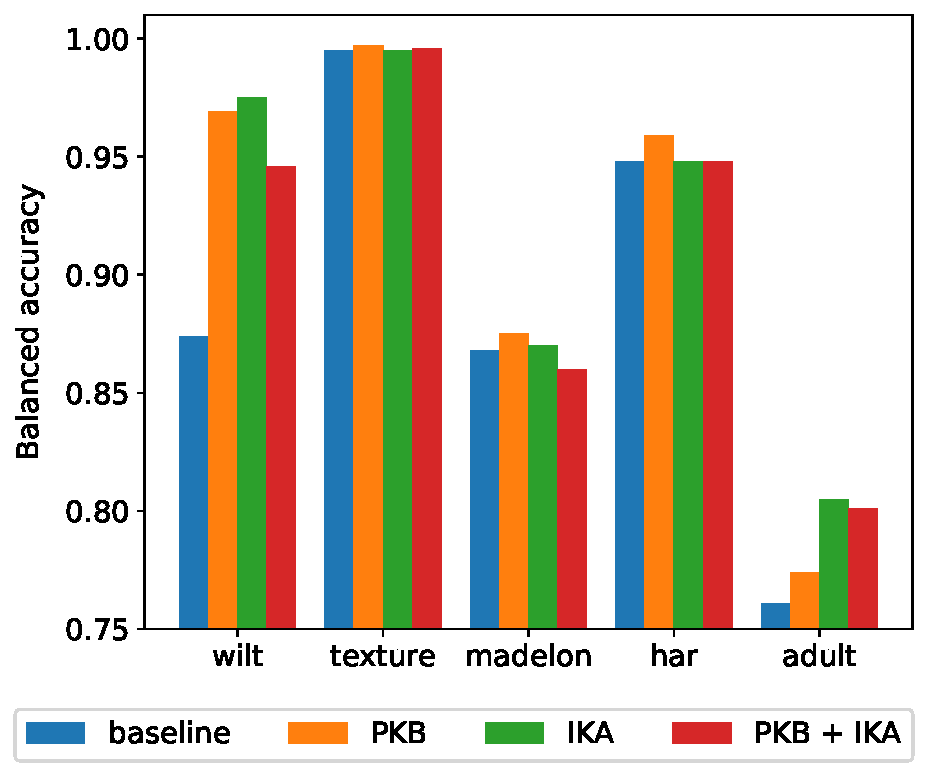
\includegraphics[scale=.45]{chapters/human-centric/hamlet/img/accuracy.pdf}
    \caption{Results assessing the effectiveness of HAMLET w.r.t. the baseline.}
    \label{hamlet-fig:effectiveness}
\end{figure}

\begin{figure}[h!]
    \RawFloats
    \centering
    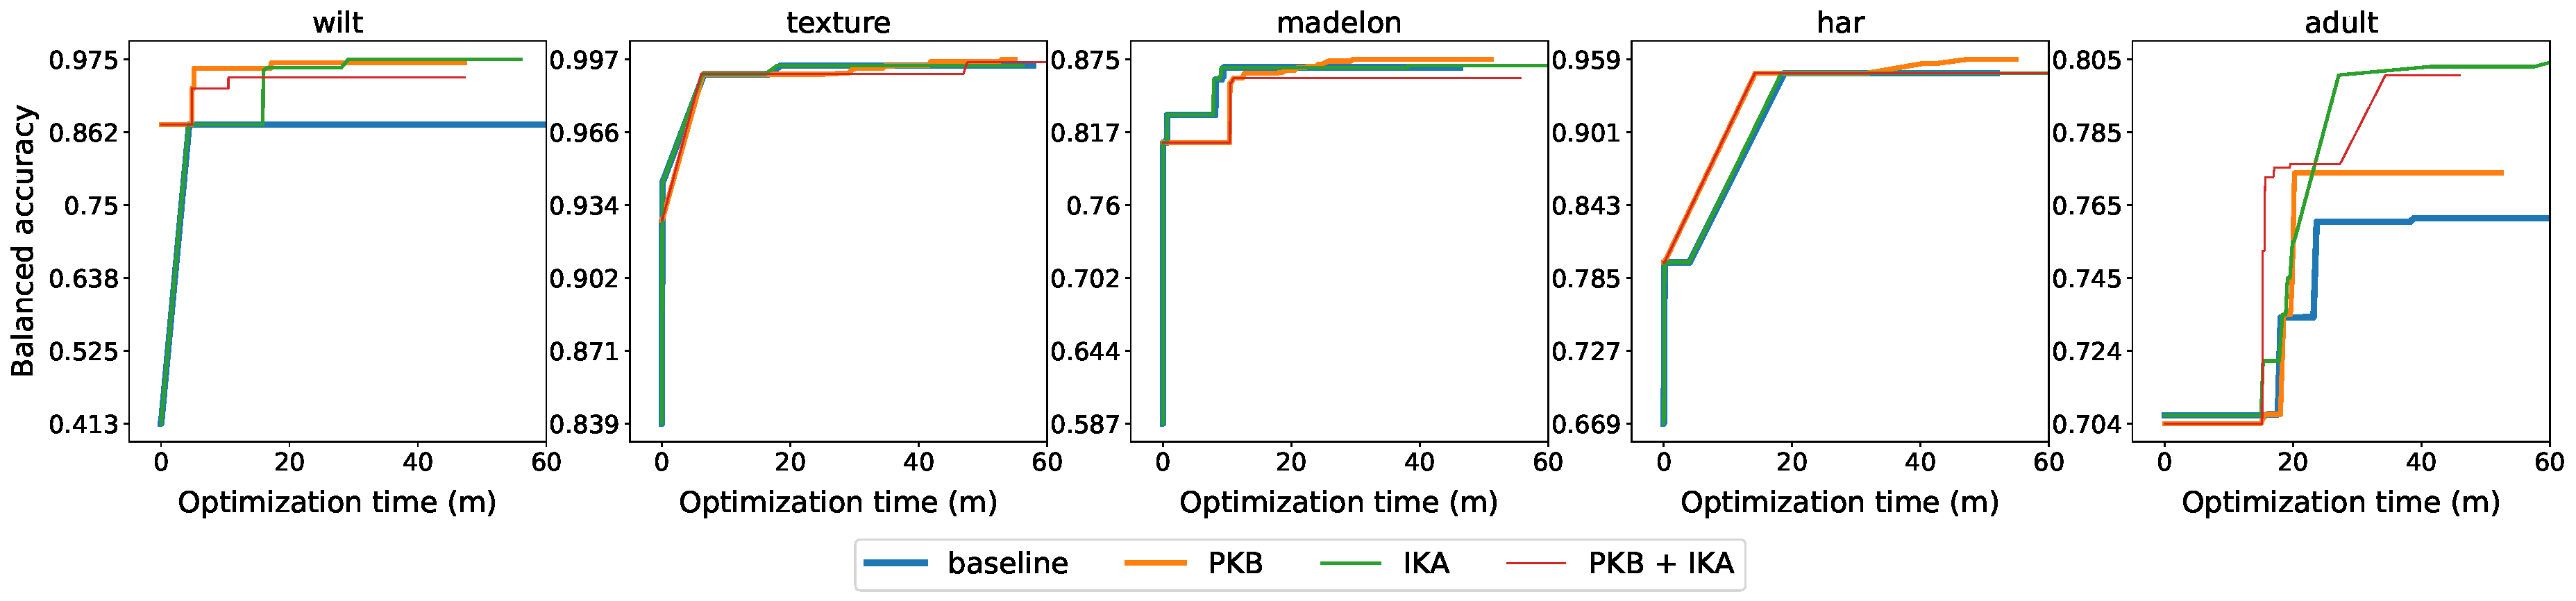
\includegraphics[scale=.25]{chapters/human-centric/hamlet/img/accuracy_time.pdf}
    \caption{Results assessing the performance of HAMLET through the optimization time.}
    \label{hamlet-fig:efficiency}
    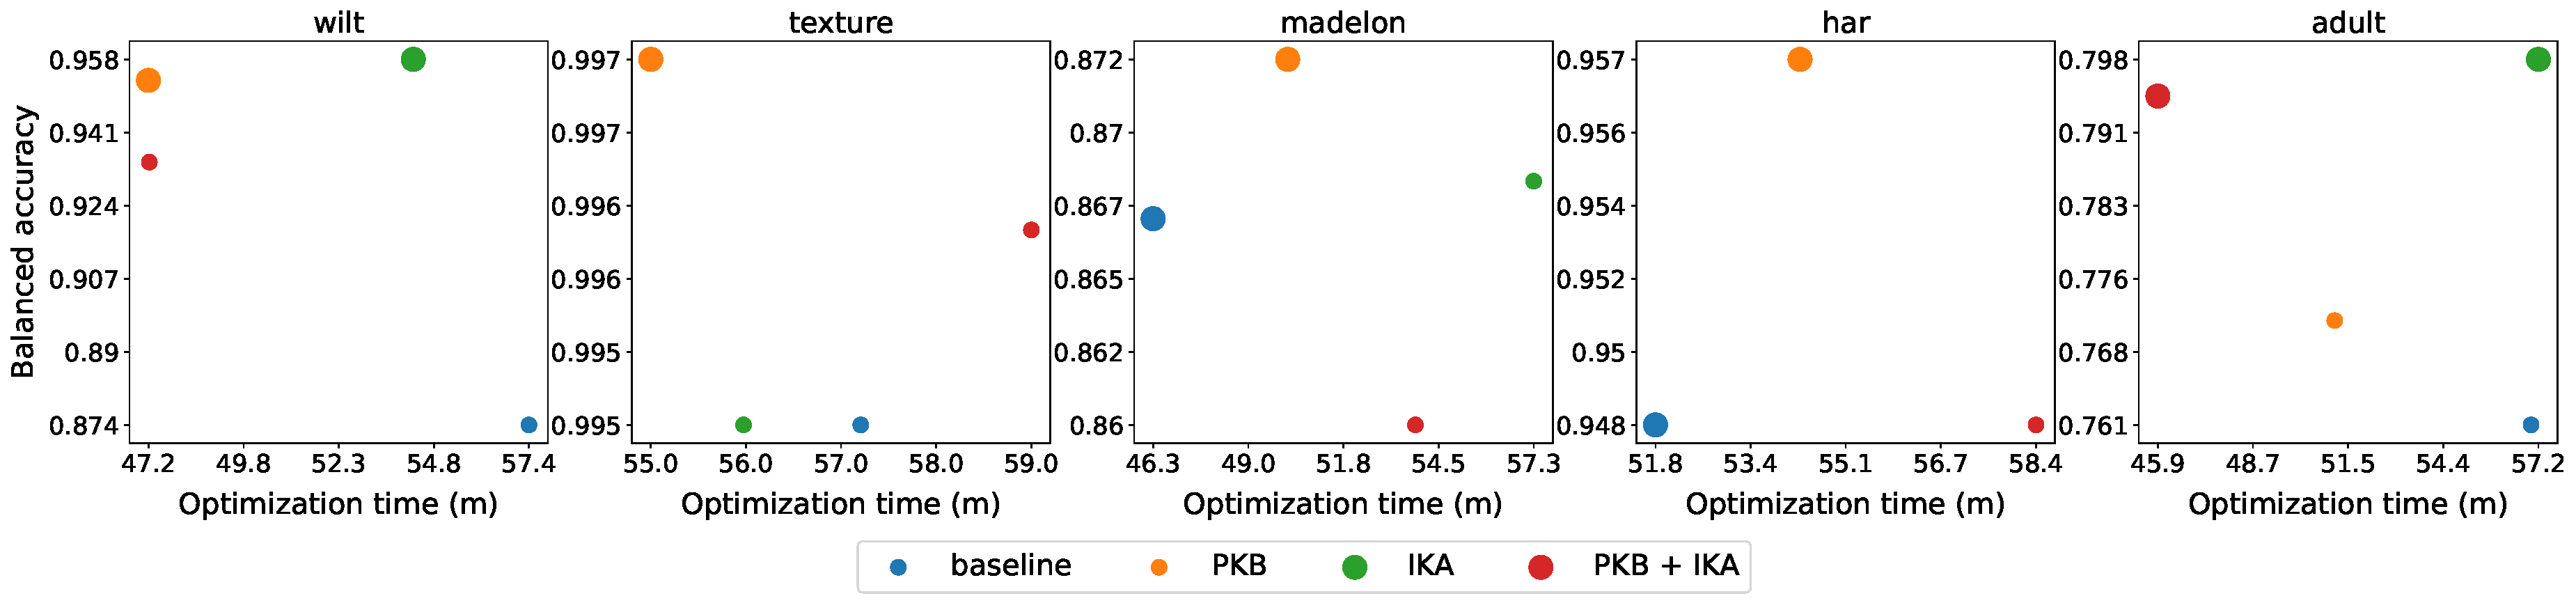
\includegraphics[scale=.25]{chapters/human-centric/hamlet/img/skyline.pdf}
    \caption{Comparison of the best pipeline instances characterized by optimization time and (balanced) accuracy, bigger circles represent settings that dominate the others.}
    \label{hamlet-fig:effskyline}
\end{figure}

We employ balanced accuracy as the quality metric.
For instance, in case of (two) binary classes, such a score is
$$
\texttt{Balanced accuracy} = \frac{1}{2}\left ( \frac{TP}{TP + FN} + \frac{TN}{TN + FP}\right )
$$
where $TP$ and $TN$ stand respectively for True Positive and True Negative (i.e., number of instances that have been correctly assigned to the positive and negative classes), and $FP$ and $FN$ stand respectively for False Positive and False Negative (i.e., number of instances that have been mistakenly assigned to the positive and negative classes). The formulation generalized to more than 2 classes can be found at \cite{DBLP:conf/icpr/BrodersenOSB10}.
The score avoids inflated performance estimations on imbalanced datasets.
For balanced datasets, the score is equal to the conventional accuracy (i.e., the number of correct predictions divided by the total number of predictions), otherwise it drops to $\frac{1}{\#classes}$.

\Cref{hamlet-fig:effectiveness} illustrates the performance achieved by the baseline and the three settings of HAMLET.
HAMLET is clearly beneficial since in all datasets the framework overcomes the baseline.
The preliminary results highlight that both the LogicalKB and rule recommendation play important roles:
\begin{itemize}
    \item When we warm-start the exploration with a non-empty LogicalKB (PKB), in all datasets HAMLET overcomes the baseline.
    \item When we only leverage rule recommendation (IKA), we achieve results that are better than or equivalent to PKB, indeed we are injecting in the LogicalKB new rules that are tailored to the dataset.
    \item The synergy of PKB+IKA performs better than PKB in adult, worse in wilt, and the two are comparable in the other datasets.
    On the one hand, the PKB act as a warm start mechanism that speeds up the optimization; on the other hand, if not aligned with the recommended rules, it can mitigate the benefits of IKA.
    This proves to be a promising direction that further requires investigation since merging the words will require further studies.
    Indeed, it is worth noting that the recommended rules can be overlapping with the ones in the LogicalKB, highlighting the need to improve the recommendation process by also considering the rules that are already present in the LogicalKB.
\end{itemize}

In PKB+IKA, IKA can introduce rules that contradict the ones in the LogicalKB of PKB; for instance when the PKB contains rules that are not ``representative'' of the dataset/algorithms in use. We believe that this is an added value of HAMLET since ``incomplete'' (or even wrong) LogicalKBs can be corrected/refined by a data-driven approach. Finally, PKB+IKA and IKA are likely to produce different rules, since in PKB+IKA the LogicalKB biases the exploration of the search space from the beginning (acting as a warm start mechanism).

\subsection{Efficiency}


\Cref{hamlet-fig:efficiency} shows how settings converge to the optimal pipeline instance.
Noticeably, PKB and PKB+IKA start with higher accuracy than IKA and the baseline in four datasets out of five, proving how the preliminary LogicalKB warm starts the exploration.
However, time and \#iterations alone are not fair metrics for comparison; for instance, an optimization strategy could privilege simple algorithms taking small amounts of computational time but producing worse results than ``more complex'' algorithms.
In the direction of multi-objective optimization (exploration time should be minimized while accuracy should be maximized), \Cref{hamlet-fig:effskyline} depicts which settings dominate the others using the Skyline operator \cite{borzsony2001skyline}.
A setting dominates another one if it is as good or better in all dimensions (time and accuracy) and better in at least one dimension (time or accuracy).
PKB dominates in 80\% of the datasets, IKA in 40\%, PKB+IKA in 20\%, and the baseline in 40\%.
Noticeably, the baseline is selected as dominating only in madelon and har datasets due to the fact that converges faster than HAMLET (although it converges to a pipeline instance with lower accuracy).


\begin{figure}[t]
    \centering
    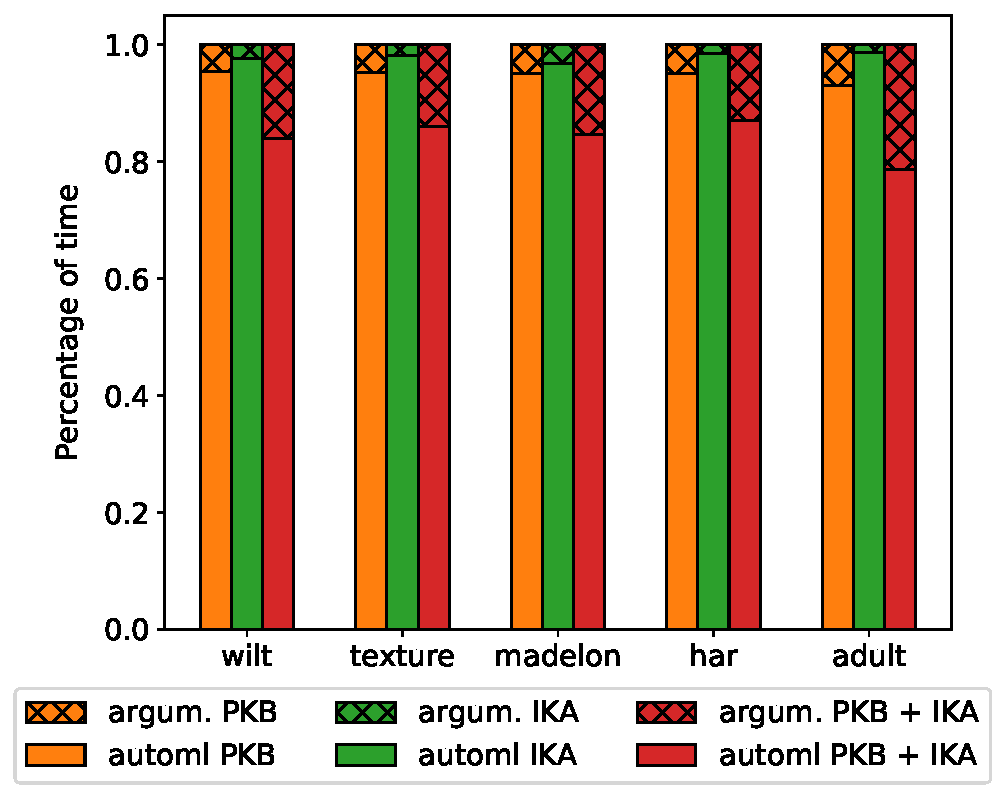
\includegraphics[scale=.43]{chapters/human-centric/hamlet/img/time.pdf}
    \caption{Computational time of the argumentation and AutoML processes.}
    \label{hamlet-fig:effoverhead}
\end{figure}


Finally, \Cref{hamlet-fig:effoverhead} depicts the overhead introduced by the argumentation framework in HAMLET that, at maximum, is 20\% of the computational time in the adult dataset.
This proves that the argumentation time is marginal with respect to the duration of the optimization process.
As expected, PKB+IKA shows the highest overhead since the number of rules to manage is the highest.

\subsection{Comparison}

\begin{figure}[t]
    \centering
    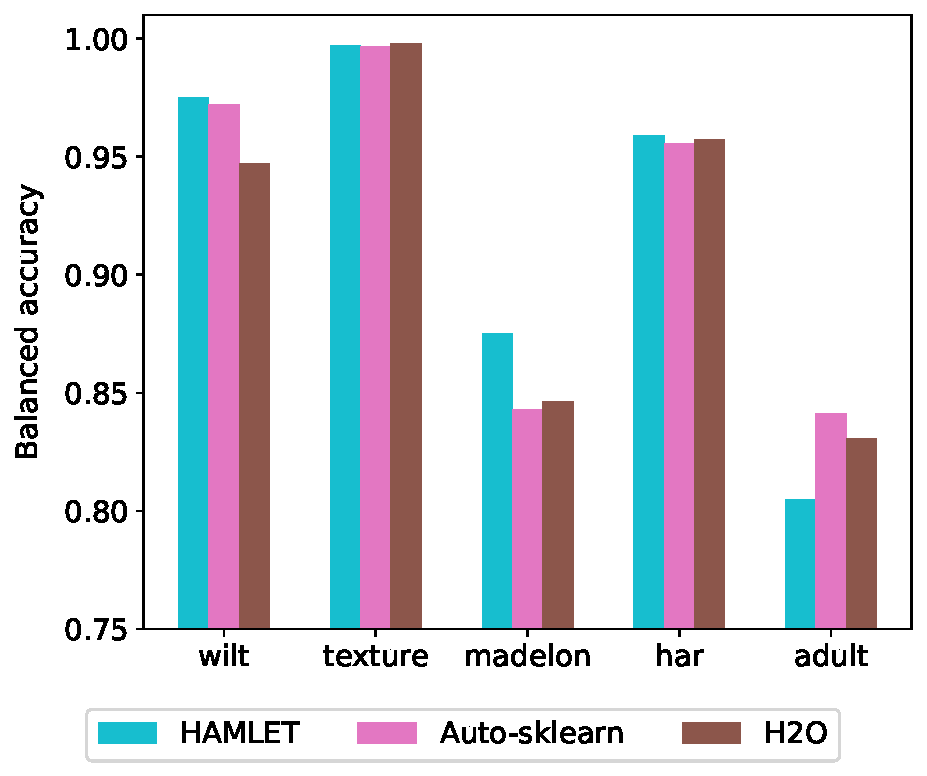
\includegraphics[scale=.45]{chapters/human-centric/hamlet/img/comparison.pdf}
    \caption{Results assessing the performance of HAMLET w.r.t. Auto-sklearn \cite{feurer2019auto} and H2O \cite{ledell2020h2o}.}
    \label{hamlet-fig:comparison}
\end{figure}


\Cref{hamlet-fig:comparison} compares HAMLET against two well-known AutoML frameworks: Auto-sklearn \cite{feurer2019auto} and H2O \cite{ledell2020h2o}.
In four datasets out of five, HAMLET outperforms or is comparable to the two frameworks.
Additionally, the added value of HAMLET is \textit{explainability}.
Hamlet is a human-in-the-loop AutoML framework tailored to the needs of data scientist that (i) enables the injection of their experience into the exploration process as well as (ii) the spreading and sharing of knowledge bases that encode what data scientists have understood by the optimization of their pipelines.


\section{Conclusions and Future Work}\label{hamlet-sec:conclusion}

Data platforms support Data Scientists in performing end-to-end data analysis; to this end, Machine Learning plays a primary role.
However, the complexity and heterogeneity of (Automated) Machine Learning processes are leading Data Scientists to lose control over such processes.
Human awareness about the constraints and solutions of Machine Learning tasks is a fundamental aspect to consider, and consequently, the Data Scientist should play a central role in the design of next-generation data platforms.

According to this vision, we present HAMLET, a framework for Human-centered AutoML based on Logic and Structured Argumentation.
Logic is exploited to structure the knowledge that the Data Scientist gathers while designing, modeling, and deploying a solution.
The logical encoding of the knowledge provides a medium that is both human- and machine-readable and it allows an easy exploration and verification of all the constraints that may apply to the case at hand---it is overwhelming for the Data Scientist to correctly handle the vast amount of them.
The preliminary evaluation of HAMLET shows promising results against state-of-the-art AutoML algorithms both in terms of effectiveness and efficiency, with argumentation introducing a small overhead with respect to the duration of the exploration process.

The directions for future work are plentiful, among them:
\begin{itemize}
    \item[(i)] the recommendation of more constraints out of the explored search space (e.g., rare or negative patterns);
    \item[(ii)] the support to heterogeneous constraints on hyperparameter domains;
    \item[(iii)] the injection of meta-learning into our Logical Knowledge Base to better identify when and how the constraints should be applied (e.g., this can be done after testing HAMLET on a multitude of datasets);
    \item[(iv)] the introduction of a visual metaphor (e.g., based on the Problem Graph) to help Data Scientists' understanding;
    \item[(v)] the study of automatic resolution/recommendation of conflicting constraints, also depending on the rules already embedded in the Logical Knowledge Base.
\end{itemize}
